\subsection{ArcFace}
\subsubsection{Bài toán}
Các mạng học sâu giải quyết các bài toán phân lớp gương mặt thường sử dụng hàm lỗi softmax để tính xác suất của một ảnh gương mặt thuộc về đối tượng nào. Nhưng khi số lượng ảnh trong cơ sở dữ liệu tăng đáng kể ngày nay, hàm softmax khó có thể phân biệt các điểm dữ liệu ở gần biên của 2 đối tượng khác nhau.\\
ArcFace sử dụng hàm lỗi Additive Angular Margin với mục tiêu gom các ảnh cùng một đối tượng lại gần nhau và các cụm đối tượng khác nhau sẽ xa nhau trong không gian latent space. Từ đó, tăng được độ hiệu quả trong các bài toán nhận dạng mặt người.\\
ArcFace là một giải pháp được phát triển bởi InsightFace - một dữ án open source cung cấp thư viện các thuật toán nhận dạng gương mặt 2D và 3D. Được trình bài trong bài báo "Additive Angular Margin Loss for Deep Face Recognition" được đăng tải trên \textit{arxiv.org} vào 23/01/2018.\\
Đối tượng tiềm năng cho giải pháp này là các hệ thống an ninh của chính phủ, khi cần quản lý rất nhiêu các đối tượng khác nhau. Hơn thế, đôi khi có các đối tượng có gương mặt khá giống nhau khiến cho khoảng cách giữa chúng trong latent space khá gần nhau dẫn đến khó nhận dạng.\\
Ta có thể tìm thấy các thông tin về ArcFace như demo minh họa, bài báo khoa học, mã nguồn tại trang \url{https://insightface.ai/arcface}
\subsubsection{Tính năng chủ đạo}
Tính năng chủ đạo của giải pháp là gom các embedding của cùng một đối tượng lại gần nhau và tách rời các cụm đối tượng ra xa nhau. Cụ thể thuật toán hoạt đông như sau:

\textit{ArcFace} đã đưa ra ý tưởng sử dụng các vector tham số làm tâm của các lớp và từ đó tối ưu "khoảng cách" giữa các điểm dữ liệu đến tâm của nó. Ta có thể hình dung được rõ hơn qua công thức sau đây:
\begin{equation}
    W_{j}^{T}x_i = \|W_j\|\cdot\|x_i\|\cos{\theta_j}
\end{equation}

Với $W_j$ là vector tham số tương ứng với lớp thứ j, $x_i$ là điểm dữ liệu và $\theta_j$ là giữa giữa $W_j$ và $x_i$.  

Ta thực hiện chuẩn hóa ($L_2$ normalisation) lên các vector $W_j$ và $x_i$. Và nhân các $x_i$ với 1 lượng s. Bằng cách chuẩn hoán như trên, ta sẽ có $\|W_j\|=1$ và $\|x_i\|=s$, nhờ đó mà dự đoán khi phân lớp chỉ phụ thuộc vào $\theta_j$. Công thức (7) được đổi thành:  
\begin{equation}
L_2=-\frac{1}{N}\sum_{i=1}^{N}{\log{\frac{e^{s\cos{\theta_{y_i}}}}{e^{s\cos{\theta_{y_i}}} + \sum_{j=1,j\neq y_i}^{N}{e^{s\cos{\theta_{j}}}}}}}
\end{equation}

Từ (10), ta có thể hình dung ra các embedding sẽ tập trung xung quanh các tâm của lớp và phân bố trên 1 mặt siêu cầu (\textit{hypersphere}). Sau đó, ta cộng một siêu tham số \textit{m (Additive Angular Margin)} vào góc giữa $x_i$ và $W_j$ để có thể tối ưu tốt hơn các khoảng cách giữa các embedding. Minh hoạ bằng hình bên dưới, ta thấy khi sử dụng hàm \textit{Softmax loss} để phân lớp, đường ranh giới giữa các lớp rất mờ, khiến cho việc phân lớp cho các điểm gần ranh giới này dễ xảy ra sai sót. Còn đối với \textit{Additive angular margin loss} bằng các sử dụng margin để ngăn cách giữa các lớp, Các điểm dữ liệu co cụm lại gần tâm của nó để  lại một khoảng cách xa giữa các lớp từ đó giúp quá trình phân lớp ít lỗi hơn.

\begin{figure}[H]
    \begin{center}
        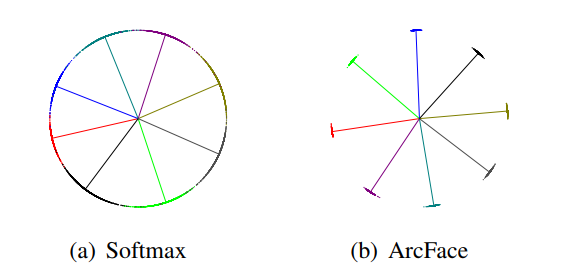
\includegraphics[scale=0.5]{images/ex2/softmax-vs-arcface}
        \caption{So sánh giữa softmax và afcface}
    \end{center}
\end{figure}

\textbf{Ưu điểm}
\begin{itemize}
	\item Độ phức tạp thấp, hiệu suất cao, lập trình dễ dàng.
	\item Có độ hội tụ tốt trên các tập dữ liệu khác nhau mà không cần kết hợp thêm hàm độ lỗi nào khác.
\end{itemize}
\textbf{Nhược điểm}
\begin{itemize}
	\item Khi số lượng các lớp tăng lên thì ma trận W cũng sẽ tăng lên đáng kể.
	\item Sử dụng hàm arccos khi chi phí tính toán chưa tối ưu.
\end{itemize}

\textbf{Tiềm năng phát triển}: \textit{ArcFace} đang mở ra các hướng đi mới trong việc giaỉ quyết các bài toán nhận dạng khuôn mặt với số đối tượng cần nhận dạng quá nhiều. Có thể thấy sự phát triển của giải pháp này trong quá khứ từ \textit{SphereFace} đến \textit{CosFace} và giờ là \textit{ArcFace} đang là state-of-the-art trong các bài toán nhận dang khuôn mặt. Và trong tương lai, hướng giải quyết này sẽ còn có khả năng phát triển để có thể giúp các tổ chức chính phủ quản lý người dân, thắt chặt an ninh và truy vết, bắt giữ các phần tử nguy hiểm trong xã hội nhanh chóng.

Có thể có cái nhìn tổng quát hơn về khác biệt của các độ lỗi bằng hình bên dưới, có thể thấy các phương pháp \textit{SphereFace} và \textit{CosFace} có các đường biên quyết định (\textit{decision boundary}) có dạng phi tuyến, trong khi \textit{ArcFace} lại cho kết quả tuyến tính giúp phân lớp dễ dàng hơn.  

\begin{figure}[H]
    \begin{center}
        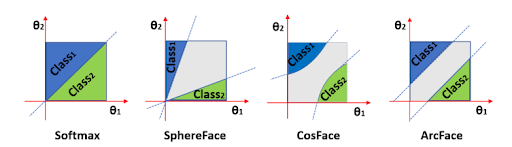
\includegraphics[scale=0.7]{images/ex2/loss-cmp}
        \caption{So sánh giữa giữa các độ lỗi}
    \end{center}
\end{figure}


